\section{Algoritmos de Grafos}
A seguir iremos abordar alguns algoritmos de grafos, para facilitar o
entendimento em geral, será optado pelo uso de pseudo-linguagem nas
explicações, seguidos dos códigos em C++ e Python.

\subsection{Algoritmos de Busca}
\input{secoes/algoritmos/3.1.1.dfs}
\newpage
\subsubsection{BFS - Breadth First Search (Busca em largura)}
A busca em largura explora o grafo nível por nível, visitando primeiro todos os
vizinhos diretos de um nó antes de avançar para os vizinhos dos vizinhos. Para
isso, utiliza uma estrutura de dados de fila (\textit{Queue} - FIFO). Sua complexidade é: $\mathcal{O}(V+E)$

\paragraph{Pseudo-Código: }\mbox{}\\
\begin{algorithm}[H]
	%linhas dos blocos if, for
	\SetAlgoLined

	\SetKwFunction{BFS}{BFS}
	\SetKwProg{Fn}{Função}{:}{}

	\Fn{\BFS{$inicio, adj$}}{
		$fila \gets$ nova Fila()\;
		$visitado \gets$ novo vetor de booleanos\;
		$fila.push(inicio)$\;
		$visitado[inicio] \gets \text{true}$\;

		\While{\text{enquanto } $fila$ \text{ não vazia}}{
			$v \gets fila.front()$; $fila.pop()$\;
			\text{processar } $v$\;

			\ParaCada{$u \in adj[v]$}{
				\Se{$\neg visitado[u]$}{
					$visitado[u] \gets \text{true}$\;
					$fila.push(u)$\;
				}
			}
		}
	}
	\caption{Busca em Largura (BFS)}
\end{algorithm}

O funcionamento da BFS garante que encontramos o caminho mais curto em grafos
não ponderados, pois ela expande as frentes de busca de forma uniforme.

Veja a BFS funcionando de maneira mais visual, iniciando em $BFS(1)$:\\
\vspace{0.5cm} \noindent % Garante que não haja recuo de parágrafo indesejado
\begin{minipage}[t]{0.31\textwidth}
	\centering
	\textbf{Passo 1: Início}\\
	\vspace{0.2cm}
	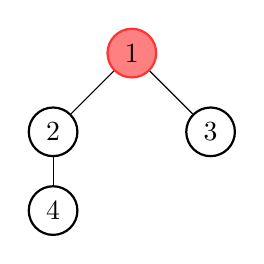
\begin{tikzpicture}[every node/.style={circle, draw, minimum size=0.5cm, thick},
			visited/.style={fill=gray!30},
			current/.style={fill=red!50, draw=red!80}]

		\node[current] (1) at (0, 1) {1};
		\node (2) at (-1, 0) {2};
		\node (3) at (1, 0) {3};
		\node (4) at (-1, -1) {4};

		\draw (1) -- (2);
		\draw (1) -- (3);
		\draw (2) -- (4);
	\end{tikzpicture}

	\vspace{0.2cm}
	\footnotesize
	\raggedright
	Insere 1 na fila. O nó 1 é o atual. Fila: [1].
\end{minipage}
\hfill
\begin{minipage}[t]{0.31\textwidth}
	\centering
	\textbf{Passo 2: Expandindo 1}\\
	\vspace{0.2cm}
	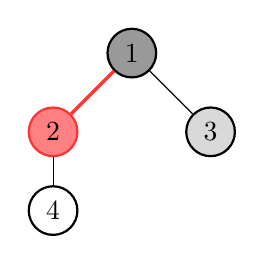
\begin{tikzpicture}[every node/.style={circle, draw, minimum size=0.5cm, thick},
			visited/.style={fill=gray!30},
			current/.style={fill=red!50, draw=red!80},
			finished/.style={fill=gray!80}]

		\node[finished] (1) at (0, 1) {1};
		\node[current] (2) at (-1, 0) {2};
		\node[visited] (3) at (1, 0) {3};
		\node (4) at (-1, -1) {4};

		\draw[very thick, red!80] (1) -- (2);
		\draw[visited] (1) -- (3);
		\draw (2) -- (4);
	\end{tikzpicture}

	\vspace{0.2cm}
	\footnotesize
	\raggedright
	Remove 1. Visita e insere os vizinhos 2 e 3 na fila. Fila: [2, 3].
\end{minipage}
\hfill
\begin{minipage}[t]{0.31\textwidth}
	\centering
	\textbf{Passo 3: Expandindo 2}\\
	\vspace{0.2cm}
	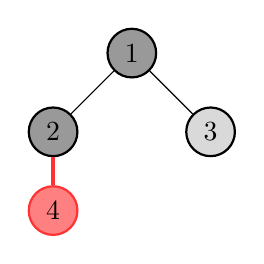
\begin{tikzpicture}[every node/.style={circle, draw, minimum size=0.5cm, thick},
			visited/.style={fill=gray!30},
			current/.style={fill=red!50, draw=red!80},
			finished/.style={fill=gray!80}]

		\node[finished] (1) at (0, 1) {1};
		\node[finished] (2) at (-1, 0) {2};
		\node[visited] (3) at (1, 0) {3};
		\node[current] (4) at (-1, -1) {4};

		\draw[finished] (1) -- (2);
		\draw[visited] (1) -- (3);
		\draw[very thick, red!80] (2) -- (4);
	\end{tikzpicture}

	\vspace{0.2cm}
	\footnotesize
	\raggedright
	Remove 2. Visita e insere o vizinho 4. Fila: [3, 4].
\end{minipage}
\vspace{0.3cm}
\noindent
\begin{center}
	\textbf{Passo 4: finalizando BFS}\\
	\vspace{0.2cm}
	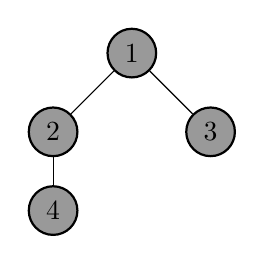
\begin{tikzpicture}[every node/.style={circle, draw, minimum size=0.5cm, thick},
			visited/.style={fill=gray!30},
			current/.style={fill=red!50, draw=red!80},
			finished/.style={fill=gray!80}]

		\node[finished] (1) at (0, 1) {1};
		\node[finished] (2) at (-1, 0) {2};
		\node[finished] (3) at (1, 0) {3};
		\node[finished] (4) at (-1, -1) {4};

		\draw[finished] (1) -- (2);
		\draw[finished] (1) -- (3);
		\draw[finished] (2) -- (4);
	\end{tikzpicture}

	\footnotesize
	\centering
	Removemos o vizinho 4 e ele não tinha vizinhos, então finalizado. E vamos remover 3 e vai ocorrer o mesmo de não ter vizinhos, logo finalizamos a BFS.
\end{center}
Veja que a ordem de visitação por níveis da BFS resulta em: $[1, 2, 3, 4]$.

\paragraph{Implementação: }\mbox{}
Vejamos a implementação da BFS em Python e em C++.

\textbf{Python: }
\begin{lstlisting}[language=Python]
	from collections import deque
	
	def bfs(inicio, adj):
	visitado = [False] * len(adj)
	fila = deque([inicio])
	visitado[inicio] = True
	
	while fila:
	v = fila.popleft()
	print(v) # Processa o vertice atual
	for u in adj[v]:
	if not visitado[u]:
	visitado[u] = True
	fila.append(u)
\end{lstlisting}

\vspace{0.3cm}
\textbf{C++:}
\begin{lstlisting}[language=C++]
	void bfs(int inicio, const vector<vector<int>>& adj) {
		vector<bool> visited(adj.size(), false);
		queue<int> q;
		
		q.push(inicio);
		visited[inicio] = true;
		
		while (!q.empty()) {
			int v = q.front();
			q.pop();
			// Processa o vertice atual aqui
			
			for (int u : adj[v]) {
				if (!visited[u]) {
					visited[u] = true;
					q.push(u);
				}
			}
		}
	}
\end{lstlisting}

\subsection{Algoritmos de Caminho Mínimo de Fonte Única}
\subsubsection{Dijkstra - Caminho Mínimo com Pesos Não Negativos}
O algoritmo de Dijkstra encontra o caminho mais curto a partir de um nó origem
para todos os outros nós em um grafo com arestas de pesos não negativos. Ele
utiliza uma Fila de Prioridade (\textit{Min-Heap}) para explorar sempre o nó
mais próximo que ainda não foi totalmente processado, garantindo uma abordagem
gulosa e eficiente. Sua complexidade é: $\mathcal{O}(E \log(V))$

\paragraph{Pseudo-Código: }\mbox{}\\
\begin{algorithm}[H]
	\SetAlgoLined
	\SetKwFunction{Dijkstra}{Dijkstra}
	\SetKwProg{Fn}{Função}{:}{}

	\Fn{\Dijkstra{$inicio, adj$}}{
		$dist \gets$ array de distâncias inicializado com $\infty$\;
		$pq \gets$ nova FilaDePrioridade()\;
		$dist[inicio] \gets 0$\;
		$pq.push((0, inicio))$\;

		\While{\text{enquanto } $pq$ \text{ não vazia}}{
			$(d, u) \gets pq.top()$; $pq.pop()$\;

			\Se{$d > dist[u]$}{
				\text{continua para a próxima iteração}\;
			}

			\ParaCada{$(peso, v) \in adj[u]$}{
				\Se{$dist[u] + peso < dist[v]$}{
					$dist[v] \gets dist[u] + peso$\;
					$pq.push((dist[v], v))$\;
				}
			}
		}
	}
	\caption{Algoritmo de Dijkstra}
\end{algorithm}

Veja o Dijkstra funcionando, encontrando o caminho mínimo a partir do nó 1:\\
\vspace{0.5cm} \noindent % Garante que não haja recuo de parágrafo indesejado
\begin{minipage}[t]{0.31\textwidth}
	\centering
	\textbf{Passo 1: Início}\\
	\vspace{0.2cm}
	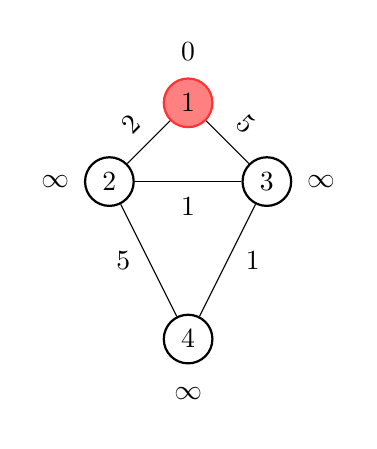
\begin{tikzpicture}[every node/.style={circle, draw, minimum size=0.5cm, thick}, visited/.style={fill=gray!30}, current/.style={fill=red!50, draw=red!80}]
		\node[current, label=above:{$0$}] (1) at (0, 1) {1};
		\node[label=left:{$\infty$}] (2) at (-1, 0) {2};
		\node[label=right:{$\infty$}] (3) at (1, 0) {3};
        \node[label=below:{$\infty$}] (4) at (0, -2) {4};
        
		\draw (1) -- node[above, sloped, draw=none, fill=none] {2} (2);
		\draw (1) -- node[above, sloped, draw=none, fill=none] {5} (3);
		\draw (2) -- node[below, draw=none, fill=none] {1} (3);
        \draw (3) -- node[right, draw=none, fill=none] {1} (4);
        \draw (2) -- node[left, draw=none, fill=none] {5} (4);
	\end{tikzpicture}

	\vspace{0.2cm}
	\footnotesize
	\raggedright
	Distância de 1 é 0. Outros são $\infty$. Fila: [(0, 1)].
\end{minipage}
\hfill
\begin{minipage}[t]{0.31\textwidth}
	\centering
	\textbf{Passo 2: Expandindo 1}\\
	\vspace{0.2cm}
	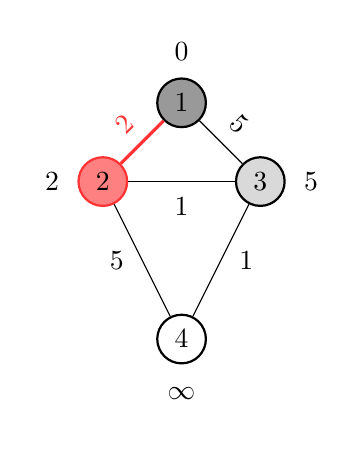
\begin{tikzpicture}[every node/.style={circle, draw, minimum size=0.5cm, thick}, visited/.style={fill=gray!30}, current/.style={fill=red!50, draw=red!80}, finished/.style={fill=gray!80}]
		\node[finished, label=above:{$0$}] (1) at (0, 1) {1};
		\node[current, label=left:{$2$}] (2) at (-1, 0) {2};
		\node[visited, label=right:{$5$}] (3) at (1, 0) {3};
        \node[label=below:{$\infty$}] (4) at (0, -2) {4};
		\draw[very thick, red!80] (1) -- node[above, draw=none, fill=none, sloped] {2} (2);
		\draw[visited] (1) -- node[above, sloped, draw=none, fill=none] {5} (3);
		\draw (2) -- node[below, draw=none, fill=none] {1} (3);
        \draw (3) -- node[right, draw=none, fill=none] {1} (4);
        \draw (2) -- node[left, draw=none, fill=none] {5} (4);
	\end{tikzpicture}

	\vspace{0.2cm}
	\footnotesize
	\raggedright
	Tira 1. Relaxa arestas. $dist[2]=2$, $dist[3]=5$. Fila: [(2, 2), (5, 3)].
\end{minipage}
\hfill
\begin{minipage}[t]{0.31\textwidth}
	\centering
	\textbf{Passo 3: Expandindo 2}\\
	\vspace{0.2cm}
	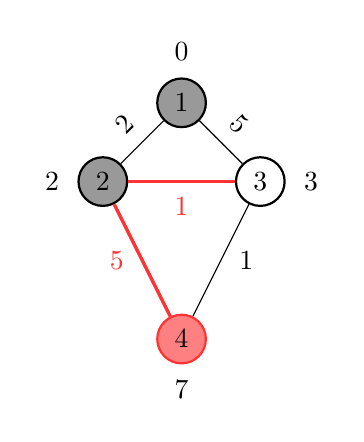
\begin{tikzpicture}[every node/.style={circle, draw, minimum size=0.5cm, thick}, visited/.style={fill=gray!30}, current/.style={fill=red!50, draw=red!80}, finished/.style={fill=gray!80}]
		\node[finished, label=above:{$0$}] (1) at (0, 1) {1};
		\node[finished, label=left:{$2$}] (2) at (-1, 0) {2};
		\node[label=right:{$3$}] (3) at (1, 0) {3};
        \node[current, label=below:{$7$}] (4) at (0, -2) {4};
        \draw[very thick, red!80] (2) -- node[left,fill=none, draw=none] {5} (4);
        \draw (3) -- node[right, draw=none, fill=none] {1} (4);
		\draw[finished] (1) -- node[above, sloped, draw=none, fill=none] {2} (2);
		\draw[visited] (1) -- node[above, sloped, draw=none, fill=none] {5} (3);
		\draw[very thick, red!80] (2) -- node[below, draw=none, fill=none] {1} (3);
	\end{tikzpicture}

	\vspace{0.2cm}
	\footnotesize
	\raggedright
	Tira 2. $2 + 1 < 5$. Atualiza $dist[3]=3$. $2+5 < \infty$, atualiza $dist[4] = 7$. Fila: [(3, 3), (5, 3), (7, 4)].
\end{minipage}
\newpage
\begin{center}
	\textbf{Passo 4: Expandindo 3}\\
	\vspace{0.2cm}
	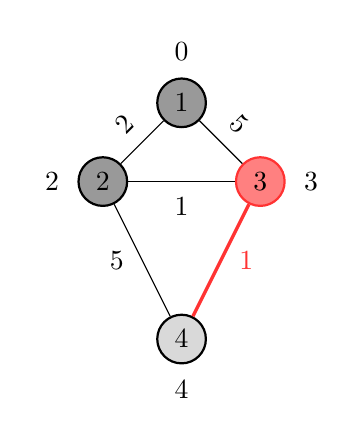
\begin{tikzpicture}[every node/.style={circle, draw, minimum size=0.5cm, thick}, visited/.style={fill=gray!30}, current/.style={fill=red!50, draw=red!80}, finished/.style={fill=gray!80}]
		\node[finished, label=above:{$0$}] (1) at (0, 1) {1};
		\node[finished, label=left:{$2$}] (2) at (-1, 0) {2};
		\node[current, label=right:{$3$}] (3) at (1, 0) {3};
        \node[visited, label=below:{$4$}] (4) at (0, -2) {4};
        
		\draw (1) -- node[above, sloped, draw=none, fill=none] {2} (2);
		\draw (1) -- node[above, sloped, draw=none, fill=none] {5} (3);
		\draw (2) -- node[below, draw=none, fill=none] {1} (3);
        \draw [very thick, red!80] (3) -- node[right, draw=none, fill=none] {1} (4);
        \draw (2) -- node[left, draw=none, fill=none] {5} (4);
	\end{tikzpicture}

	\vspace{0.2cm}
	\footnotesize
	\raggedright
	Está visitando o vizinho de 3 (4). $dist[3]+peso(3\xrightarrow{}4) < dist[4]$, isto é $3+1 < 7?$, sim então: $dist[4]=dist[3]+1$.
\end{center}
Nesse momento, não faz sentido avaliar mais os valores ainda presentes na fila de prioridade, que seriam: [(5,3), (7,4)], pois eles não iriam melhorar nenhum resultado. Pois o caminho (5,3) significa que tem peso 5 pra chegar até 3, porém isso seria descartado pela linha
\begin{lstlisting}[language=C++]
    if d>dist[u]{ 
        continue; 
    }
\end{lstlisting}
Essa linha de código serve justamente para evitar analisar relaxamentos de arestas desnecessários. 

Ao finalizar o Dijkstra nosso vetor de distâncias calculou o seguinte: 

$dist[u]$ é a distância mínima entre a origem $s$ até $u$, lembrando que para o exemplo acima a origem foi o vértice 1, então $dist[2]$ é a menor distância entre de 1 até 2. Esse algoritmo pode ser modificado, possibilitando que recriemos o caminho (basta criar um novo vetor chamado $parent$ em que $parent[u]$ guarda o vértice que levou até $u$ no menor caminho, por exemplo $parent[4]=3$, pois o caminho minímo de $1 \xrightarrow{}4$ foi $1\xrightarrow{}2\xrightarrow{}3\xrightarrow{}4$
\newpage
\paragraph{Implementação: }\mbox{}\\
Vejamos a implementação do Dijkstra em Python e C++. Note o uso de \textit{heaps} para otimização.

\textbf{Python: }
\begin{lstlisting}[language=Python]
import heapq

def dijkstra(inicio, adj, n):
    dist = [float('inf')] * n
    dist[inicio] = 0
    pq = [(0, inicio)]
    
    while pq:
        d, u = heapq.heappop(pq)
        if d > dist[u]:
            continue
            
        for peso, v in adj[u]:
            if dist[u] + peso < dist[v]:
                dist[v] = dist[u] + peso
                heapq.heappush(pq, (dist[v], v))
                
    return dist
\end{lstlisting}

\vspace{0.3cm}
\textbf{C++:}
\begin{lstlisting}[language=C++]
vector<int> dijkstra(int inicio, int n, const vector<vector<pair<int, int>>>& adj) {
    vector<int> dist(n, 1e9);
    priority_queue<pair<int, int>, vector<pair<int, int>>, greater<pair<int, int>>> pq;
    
    dist[inicio] = 0;
    pq.push({0, inicio});
    
    while (!pq.empty()) {
        int d = pq.top().first;
        int u = pq.top().second;
        pq.pop();
        
        if (d > dist[u]) continue;
        
        for (auto edge : adj[u]) {
            int peso = edge.first;
            int v = edge.second;
            
            if (dist[u] + peso < dist[v]) {
                dist[v] = dist[u] + peso;
                pq.push({dist[v], v});
            }
        }
    }
    return dist;
}
\end{lstlisting}
\subsubsection{Bellman-Ford (Caminho Mínimo com Pesos Negativos)}
O algoritmo de Bellman-Ford é utilizado para encontrar caminhos mínimos em
grafos que contêm arestas com pesos negativos. Ao contrário do Dijkstra, ele
relaxa todas as arestas do grafo repetidas vezes ($V-1$ vezes, onde $V$ é o
número de vértices). Se no $V$-ésimo passo ainda for possível relaxar alguma
aresta, significa que existe um \textbf{ciclo de peso negativo} no grafo. Sua complexidade é: $\mathcal{O}(V * E)$

\paragraph{Pseudo-Código: }\mbox{}\\
\begin{algorithm}[H]
	\SetAlgoLined
	\SetKwFunction{BellmanFord}{BellmanFord}
	\SetKwProg{Fn}{Função}{:}{}

	\Fn{\BellmanFord{$inicio, arestas, V$}}{
		$dist \gets$ array de tamanho $V$ inicializado com $\infty$\;
		$dist[inicio] \gets 0$\;

		\Para{$i \gets 1$ \Ate $V - 1$}{
			\ParaCada{$(u, v, peso) \in arestas$}{
				\Se{$dist[u] + peso < dist[v]$}{
					$dist[v] \gets dist[u] + peso$\;
				}
			}
		}

		\ParaCada{$(u, v, peso) \in arestas$}{
			\Se{$dist[u] + peso < dist[v]$}{
				\Retorna \text{Ciclo negativo detectado}\;
			}
		}
	}
	\caption{Algoritmo de BellmanFord}
\end{algorithm}

Veja uma iteração de relaxamento do Bellman-Ford:\\ \vspace{0.5cm} \noindent
\begin{minipage}[t]{0.31\textwidth}
	\centering
	\textbf{Passo 1: Estado Inicial}\\
	\vspace{0.2cm}
	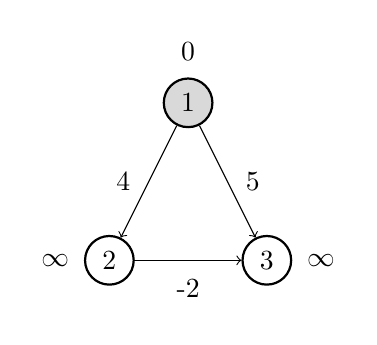
\begin{tikzpicture}[every node/.style={circle, draw, minimum size=0.5cm, thick}]
		\node[fill=gray!30, label=above:{$0$}] (1) at (0, 1) {1};
		\node[label=left:{$\infty$}] (2) at (-1, -1) {2};
		\node[label=right:{$\infty$}] (3) at (1, -1) {3};
		\draw[->] (1) -- node[left, draw=none, fill=none] {4} (2);
		\draw[->] (1) -- node[right, draw=none, fill=none] {5} (3);
		\draw[->] (2) -- node[below, draw=none, fill=none] {-2} (3);
	\end{tikzpicture}

	\vspace{0.2cm}
	\footnotesize
	\raggedright
	Distâncias iniciais: $dist[1]=0$, outros $\infty$.
\end{minipage}%
\hfill
%
\begin{minipage}[t]{0.31\textwidth}
	\centering
	\textbf{Passo 2: Relaxando 1 $\to$ 2 e 1 $\to$ 3}\\
	\vspace{0.2cm}
	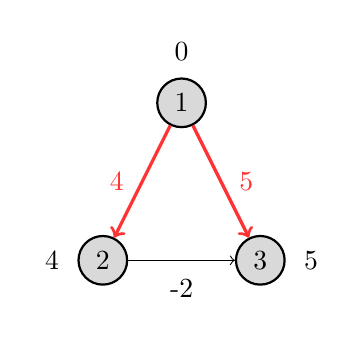
\begin{tikzpicture}[every node/.style={circle, draw, minimum size=0.5cm, thick}]
		\node[fill=gray!30, label=above:{$0$}] (1) at (0, 1) {1};
		\node[fill=gray!30, label=left:{$4$}] (2) at (-1, -1) {2};
		\node[fill=gray!30, label=right:{$5$}] (3) at (1, -1) {3};
		\draw[->, very thick, red!80] (1) -- node[left, draw=none, fill=none] {4} (2);
		\draw[->, very thick, red!80] (1) -- node[right, draw=none, fill=none] {5} (3);
		\draw[->] (2) -- node[below, draw=none, fill=none] {-2} (3);
	\end{tikzpicture}

	\vspace{0.2cm}
	\footnotesize
	\raggedright
	$dist[2] = 4$, $dist[3] = 5$.
\end{minipage}%
\hfill
%
\begin{minipage}[t]{0.31\textwidth}
	\centering
	\textbf{Passo 3: Relaxando 2 $\to$ 3}\\
	\vspace{0.2cm}
	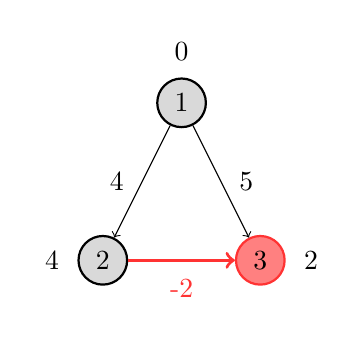
\begin{tikzpicture}[every node/.style={circle, draw, minimum size=0.5cm, thick}]
		\node[fill=gray!30, label=above:{$0$}] (1) at (0, 1) {1};
		\node[fill=gray!30, label=left:{$4$}] (2) at (-1, -1) {2};
		\node[fill=red!50, draw=red!80, label=right:{$2$}] (3) at (1, -1) {3};
		\draw[->] (1) -- node[left, draw=none, fill=none] {4} (2);
		\draw[->] (1) -- node[right, draw=none, fill=none] {5} (3);
		\draw[->, very thick, red!80] (2) -- node[below, draw=none, fill=none] {-2} (3);
	\end{tikzpicture}

	\vspace{0.2cm}
	\footnotesize
	\raggedright
	$dist[2] + (-2) < dist[3]$. Logo $dist[3] = 2$.
\end{minipage}

\paragraph{Implementação: }\mbox{}\\
\textbf{Python: }
\begin{lstlisting}[language=Python]
def bellman_ford(inicio, n, arestas):
    dist = [float('inf')] * n
    dist[inicio] = 0
    
    for _ in range(n - 1):
        for u, v, peso in arestas:
            if dist[u] != float('inf') and dist[u] + peso < dist[v]:
                dist[v] = dist[u] + peso
                
    # Verificacao de ciclo negativo
    for u, v, peso in arestas:
        if dist[u] != float('inf') and dist[u] + peso < dist[v]:
            return None 
            
    return dist
\end{lstlisting}

\vspace{0.3cm}
\textbf{C++:}
\begin{lstlisting}[language=C++]
struct Aresta {
    int u, v, peso;
};

vector<int> bellman_ford(int inicio, int n, const vector<Aresta>& arestas) {
    vector<int> dist(n, 1e9);
    dist[inicio] = 0;
    
    for (int i = 0; i < n - 1; ++i) {
        for (const auto& a : arestas) {
            if (dist[a.u] < 1e9 && dist[a.u] + a.peso < dist[a.v]) {
                dist[a.v] = dist[a.u] + a.peso;
            }
        }
    }
    
    for (const auto& a : arestas) {
        if (dist[a.u] < 1e9 && dist[a.u] + a.peso < dist[a.v]) {
            return {}; // Retorna vetor vazio se houver ciclo negativo
        }
    }
    return dist;
}
\end{lstlisting}
\newpage

\subsubsection{Floyd-Warshall (Todos os Pares)}
O algoritmo de Floyd-Warshall resolve o problema do caminho mínimo entre
\textbf{todos os pares de vértices} do grafo simultaneamente. Ele utiliza
Programação Dinâmica, avaliando se o caminho de $i$ para $j$ passando por um
vértice intermediário $k$ é menor que o caminho direto conhecido. A
complexidade de tempo é $\mathcal{O}(V^3)$.

\paragraph{Pseudo-Código: }\mbox{}\\
\begin{algorithm}[H]
    \SetAlgoLined
    \SetKwFunction{FloydWarshall}{FloydWarshall}
    \SetKwProg{Fn}{Função}{:}{}

    \Fn{\FloydWarshall{$matrizAdj, V$}}{
        $dist \gets matrizAdj$\;

        \Para{$k \gets 0$ \Ate $V - 1$}{
            \Para{$i \gets 0$ \Ate $V - 1$}{
                \Para{$j \gets 0$ \Ate $V - 1$}{
                    \Se{$dist[i][k] + dist[k][j] < dist[i][j]$}{
                        $dist[i][j] \gets dist[i][k] + dist[k][j]$\;
                    }
                }
            }
        }
    }
    \caption{Algoritmo de Floyd-Warshall}
\end{algorithm}

\paragraph{Implementação: }\mbox{}\\
\textbf{Python: }
\begin{lstlisting}[language=Python]
def floyd_warshall(n, adj_matrix):
    # Copia a matriz de adjacencia
    dist = [row[:] for row in adj_matrix]
    
    for k in range(n):
        for i in range(n):
            for j in range(n):
                if dist[i][k] + dist[k][j] < dist[i][j]:
                    dist[i][j] = dist[i][k] + dist[k][j]
                    
    return dist
\end{lstlisting}

\vspace{0.3cm}
\textbf{C++:}
\begin{lstlisting}[language=C++]
void floyd_warshall(int n, vector<vector<int>>& dist) {
    // dist ja eh inicializada com a matriz de adjacencia
    for (int k = 0; k < n; ++k) {
        for (int i = 0; i < n; ++i) {
            for (int j = 0; j < n; ++j) {
                if (dist[i][k] < 1e9 && dist[k][j] < 1e9) {
                    dist[i][j] = min(dist[i][j], dist[i][k] + dist[k][j]);
                }
            }
        }
    }
}
\end{lstlisting}

\subsection{Algoritmos de Árvores Geradoras Mínimas (MST)}
Uma Árvore Geradora Mínima (MST) de um grafo conexo, não direcionado e
ponderado é um subgrafo que é uma árvore (sem ciclos) e conecta todos os
vértices, com o menor peso total de arestas possível ($V - 1$ arestas). Veremos
a seguir os dois algoritmos clássicos para resolvê-la. \subsubsection{DSU - Disjoint Set Union (Union-Find)}
A estrutura de dados Disjoint Set Union (DSU) é utilizada para rastrear um
conjunto de elementos particionados em vários subconjuntos disjuntos (não
sobrepostos). Ela suporta duas operações principais quase em tempo constante,
$\mathcal{O}(\alpha(V))$, graças às otimizações de \textbf{compressão de
    caminho} e \textbf{união por tamanho}: a operação \textit{Find} (descobre a
qual conjunto um elemento pertence) e a \textit{Union} (une dois conjuntos).

\paragraph{Pseudo-Código: }\mbox{}\\
\begin{algorithm}[H]
    \SetAlgoLined
    \SetKwFunction{Find}{Find}
    \SetKwFunction{Union}{Union}
    \SetKwProg{Fn}{Função}{:}{}

    \Fn{\Find{$x$}}{
        \Se{$pai[x] == x$}{
            \Retorna $x$\;
        }
        $pai[x] \gets$ \Find{$pai[x]$} \text{ // Compressão de caminho}\;
        \Retorna $pai[x]$\;
    }

    \vspace{0.2cm}

    \Fn{\Union{$x, y$}}{
        $raizX \gets$ \Find{$x$}\;
        $raizY \gets$ \Find{$y$}\;

        \Se{$raizX \neq raizY$}{
            \text{// União por tamanho (liga o menor ao maior)}\;
            \Se{$tamanho[raizX] < tamanho[raizY]$}{
                \text{Trocar os valores de } $raizX$ \text{ e } $raizY$\;
            }
            $pai[raizY] \gets raizX$\;
            $tamanho[raizX] \gets tamanho[raizX] + tamanho[raizY]$\;
        }
    }
    \caption{Disjoint Set Union (DSU)}
\end{algorithm}

Veja a estrutura do DSU sendo formada (as setas apontam para o pai):\\
\vspace{0.5cm} \noindent
\begin{minipage}[t]{0.31\textwidth}
    \centering
    \textbf{Passo 1: Inicialização}\\
    \vspace{0.2cm}
    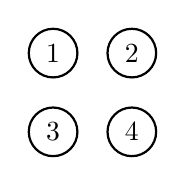
\begin{tikzpicture}[every node/.style={circle, draw, minimum size=0.5cm, thick}]
        \node (1) at (0, 0) {1};
        \node (2) at (1, 0) {2};
        \node (3) at (0, -1) {3};
        \node (4) at (1, -1) {4};
    \end{tikzpicture}

    \vspace{0.2cm}
    \footnotesize
    \raggedright
    Cada elemento é seu próprio pai. Nenhum conjunto foi unido ainda.
\end{minipage}%
\hfill
%
\begin{minipage}[t]{0.31\textwidth}
    \centering
    \textbf{Passo 2: Union(1, 2) e Union(3, 4)}\\
    \vspace{0.2cm}
    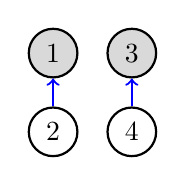
\begin{tikzpicture}[every node/.style={circle, draw, minimum size=0.5cm, thick}]
        \node[fill=gray!30] (1) at (0, 0) {1};
        \node (2) at (0, -1) {2};
        \node[fill=gray!30] (3) at (1, 0) {3};
        \node (4) at (1, -1) {4};
        \draw[->, thick, blue] (2) -- (1);
        \draw[->, thick, blue] (4) -- (3);
    \end{tikzpicture}

    \vspace{0.2cm}
    \footnotesize
    \raggedright
    1 e 3 tornam-se raízes dos seus respectivos conjuntos.
\end{minipage}%
\hfill
%
\begin{minipage}[t]{0.31\textwidth}
    \centering
    \textbf{Passo 3: Union(1, 3)}\\
    \vspace{0.2cm}
    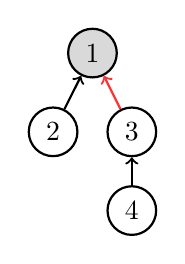
\begin{tikzpicture}[every node/.style={circle, draw, minimum size=0.5cm, thick}]
        \node[fill=gray!30] (1) at (0.5, 0) {1};
        \node (2) at (0, -1) {2};
        \node (3) at (1, -1) {3};
        \node (4) at (1, -2) {4};
        \draw[->, thick] (2) -- (1);
        \draw[->, thick, red!80] (3) -- (1);
        \draw[->, thick] (4) -- (3);
    \end{tikzpicture}

    \vspace{0.2cm}
    \footnotesize
    \raggedright
    Ambos tinham tamanho 2. O nó 1 se torna o pai do nó 3. Todos agora no mesmo conjunto.
\end{minipage}

\paragraph{Implementação: }\mbox{}
\textbf{Python: }
\begin{lstlisting}[language=Python]
class DSU:
    def __init__(self, n):
        self.pai = list(range(n))
        self.tamanho = [1] * n
        
    def find(self, x):
        if self.pai[x] == x:
            return x
        # Compressao de caminho
        self.pai[x] = self.find(self.pai[x])
        return self.pai[x]
        
    def union(self, x, y):
        raiz_x = self.find(x)
        raiz_y = self.find(y)
        
        if raiz_x != raiz_y:
            # Uniao por tamanho
            if self.tamanho[raiz_x] < self.tamanho[raiz_y]:
                raiz_x, raiz_y = raiz_y, raiz_x
                
            self.pai[raiz_y] = raiz_x
            self.tamanho[raiz_x] += self.tamanho[raiz_y]
            return True # Ocorreu uniao
        return False # Ja estavam no mesmo conjunto
\end{lstlisting}

\vspace{0.3cm}
\textbf{C++:}
\begin{lstlisting}[language=C++]
struct DSU {
    vector<int> pai, tamanho;
    
    DSU(int n) {
        pai.resize(n);
        tamanho.assign(n, 1);
        iota(pai.begin(), pai.end(), 0); // Preenche 0, 1, ..., n-1
    }
    
    int find(int x) {
        if (pai[x] == x) return x;
        return pai[x] = find(pai[x]); // Compressao de caminho
    }
    
    bool unite(int x, int y) {
        int raizX = find(x);
        int raizY = find(y);
        
        if (raizX != raizY) {
            // Uniao por tamanho
            if (tamanho[raizX] < tamanho[raizY]) swap(raizX, raizY);
            pai[raizY] = raizX;
            tamanho[raizX] += tamanho[raizY];
            return true;
        }
        return false;
    }
};
\end{lstlisting}
\newpage
\subsubsection{Kruskal (Baseado em DSU e Ordenação de Arestas)}
O algoritmo de Kruskal ordena todas as arestas do grafo em ordem crescente de
peso. Em seguida, itera por cada aresta utilizando uma estrutura de DSU: se os
vértices da aresta pertencem a conjuntos diferentes, nós os unimos e
adicionamos a aresta à MST. Caso contrário, a aresta é descartada para evitar
ciclos. A complexidade de tempo é $\mathcal{O}(E \log E)$ devido à ordenação
das arestas.

\paragraph{Pseudo-Código: }\mbox{}\\
\begin{algorithm}[H]
    \SetAlgoLined
    \SetKwFunction{Kruskal}{Kruskal}
    \SetKwProg{Fn}{Função}{:}{}

    \Fn{\Kruskal{$arestas, V$}}{
        $mst \gets \emptyset$\;
        \text{Ordenar } $arestas$ \text{ em ordem crescente de peso}\;
        \text{Inicializar } $dsu$ \text{ com } $V$ \text{ elementos}\;

        \ParaCada{$(peso, u, v) \in arestas$}{
            \Se{$dsu.find(u) \neq dsu.find(v)$}{
                $dsu.unite(u, v)$\;
                $mst.add((u, v, peso))$\;
            }
        }
        \Retorna $mst$\;
    }
    \caption{Algoritmo de Kruskal}
\end{algorithm}

Veja o Kruskal funcionando, selecionando arestas em ordem crescente de peso sem
formar ciclos:\\ \vspace{0.5cm} \noindent
\begin{minipage}[t]{0.31\textwidth}
    \centering
    \textbf{Passo 1: Arestas Ordenadas}\\
    \vspace{0.2cm}
    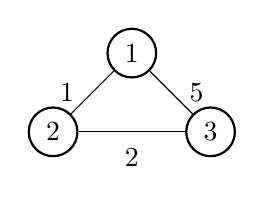
\begin{tikzpicture}[every node/.style={circle, draw, minimum size=0.5cm, thick}]
        \node (1) at (0, 1) {1};
        \node (2) at (-1, 0) {2};
        \node (3) at (1, 0) {3};
        \draw (1) -- node[left, draw=none, fill=none] {1} (2);
        \draw (2) -- node[below, draw=none, fill=none] {2} (3);
        \draw (1) -- node[right, draw=none, fill=none] {5} (3);
    \end{tikzpicture}

    \vspace{0.2cm}
    \footnotesize
    \raggedright
    Arestas ordenadas por peso: (1-2, peso 1), (2-3, peso 2), (1-3, peso 5).
\end{minipage}%
\hfill
%
\begin{minipage}[t]{0.31\textwidth}
    \centering
    \textbf{Passo 2: Adiciona aresta (1-2)}\\
    \vspace{0.2cm}
    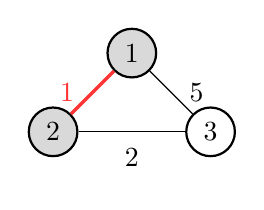
\begin{tikzpicture}[every node/.style={circle, draw, minimum size=0.5cm, thick}]
        \node[fill=gray!30] (1) at (0, 1) {1};
        \node[fill=gray!30] (2) at (-1, 0) {2};
        \node (3) at (1, 0) {3};
        \draw[very thick, red!80] (1) -- node[left, draw=none, fill=none] {1} (2);
        \draw (2) -- node[below, draw=none, fill=none] {2} (3);
        \draw (1) -- node[right, draw=none, fill=none] {5} (3);
    \end{tikzpicture}

    \vspace{0.2cm}
    \footnotesize
    \raggedright
    Menor peso (1). Unimos 1 e 2 via DSU. Aresta aceita na MST.
\end{minipage}%
\hfill
%
\begin{minipage}[t]{0.31\textwidth}
    \centering
    \textbf{Passo 3: Adiciona (2-3)}\\
    \vspace{0.2cm}
    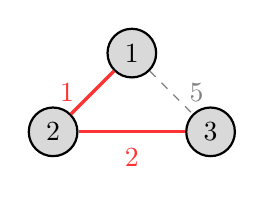
\begin{tikzpicture}[every node/.style={circle, draw, minimum size=0.5cm, thick}]
        \node[fill=gray!30] (1) at (0, 1) {1};
        \node[fill=gray!30] (2) at (-1, 0) {2};
        \node[fill=gray!30] (3) at (1, 0) {3};
        \draw[very thick, red!80] (1) -- node[left, draw=none, fill=none] {1} (2);
        \draw[very thick, red!80] (2) -- node[below, draw=none, fill=none] {2} (3);
        \draw[dashed, gray] (1) -- node[right, draw=none, fill=none] {5} (3);
    \end{tikzpicture}

    \vspace{0.2cm}
    \footnotesize
    \raggedright
    Próxima menor (2). Unimos 2 e 3. Aresta (1-3) é ignorada (formaria ciclo). MST pronta! Custo: 3.
\end{minipage}

\vspace{0.3cm}

\paragraph{Implementação: }\mbox{}\\
\textbf{Python: }
\begin{lstlisting}[language=Python]
def kruskal(n, arestas):
    # arestas = lista de tuplas (peso, u, v)
    arestas.sort()
    dsu = DSU(n)
    mst = []
    custo_total = 0
    
    for peso, u, v in arestas:
        if dsu.unite(u, v):
            mst.append((u, v, peso))
            custo_total += peso
            
    return custo_total, mst
\end{lstlisting}

\vspace{0.3cm}
\textbf{C++:}
\begin{lstlisting}[language=C++]
struct Aresta {
    int u, v, peso;
    bool operator<(const Aresta& outro) const {
        return peso < outro.peso;
    }
};

int kruskal(int n, vector<Aresta>& arestas) {
    sort(arestas.begin(), arestas.end());
    DSU dsu(n);
    int custoTotal = 0;
    
    for (auto& a : arestas) {
        if (dsu.unite(a.u, a.v)) {
            custoTotal += a.peso;
        }
    }
    return custoTotal;
}
\end{lstlisting}
\newpage 
\subsubsection{Prim (Baseado em Fila de Prioridade)}
O algoritmo de Prim constrói a MST incrementalmente a partir de um vértice
inicial arbitrário. A cada passo, ele escolhe a aresta de menor peso que
conecta um vértice que já está na MST a um vértice que ainda não está,
utilizando uma Fila de Prioridade (\textit{Min-Heap}). Sua complexidade de
tempo é $\mathcal{O}(E \log V)$.

\paragraph{Pseudo-Código: }\mbox{}\\
\begin{algorithm}[H]
    \SetAlgoLined
    \SetKwFunction{Prim}{Prim}
    \SetKwProg{Fn}{Função}{:}{}

    \Fn{\Prim{$adj, V$}}{
        $visitado \gets$ vetor de booleanos falso de tamanho $V$\;
        $pq \gets$ nova FilaDePrioridade() \text{guardando } $(peso, u)$\;
        $pq.push((0, 0))$ \text{ // Começa do vértice 0}\;
        $custoTotal \gets 0$\;

        \While{\text{enquanto } $pq$ \text{ não vazia}}{
            $(peso, u) \gets pq.top()$; $pq.pop()$\;
            \Se{$visitado[u]$}{
                \text{continuar}\;
            }
            $visitado[u] \gets \text{true}$\;
            $custoTotal \gets custoTotal + peso$\;

            \ParaCada{$(pesoVizinho, v) \in adj[u]$}{
                \Se{$\neg visitado[v]$}{
                    $pq.push((pesoVizinho, v))$\;
                }
            }
        }
        \Retorna $custoTotal$\;
    }
    \caption{Algoritmo de Prim}
\end{algorithm}

Veja o Prim crescendo a árvore a partir do vértice 1:\\ \vspace{0.5cm}
\noindent
\begin{minipage}[t]{0.31\textwidth}
    \centering
    \textbf{Passo 1: Início no Nó 1}\\
    \vspace{0.2cm}
    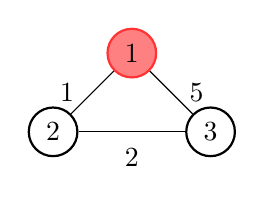
\begin{tikzpicture}[every node/.style={circle, draw, minimum size=0.5cm, thick}]
        \node[fill=red!50, draw=red!80] (1) at (0, 1) {1};
        \node (2) at (-1, 0) {2};
        \node (3) at (1, 0) {3};
        \draw (1) -- node[left, draw=none, fill=none] {1} (2);
        \draw (1) -- node[right, draw=none, fill=none] {5} (3);
        \draw (2) -- node[below, draw=none, fill=none] {2} (3);
    \end{tikzpicture}

    \vspace{0.2cm}
    \footnotesize
    \raggedright
    Inicia no vértice 1. Fila de prioridade guarda arestas incidentes: [(1, 2), (5, 3)].
\end{minipage}%
\hfill
%
\begin{minipage}[t]{0.31\textwidth}
    \centering
    \textbf{Passo 2: Expande para o Nó 2}\\
    \vspace{0.2cm}
    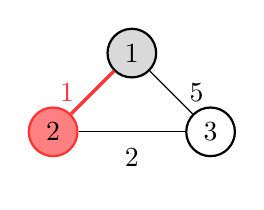
\begin{tikzpicture}[every node/.style={circle, draw, minimum size=0.5cm, thick}]
        \node[fill=gray!30] (1) at (0, 1) {1};
        \node[fill=red!50, draw=red!80] (2) at (-1, 0) {2};
        \node (3) at (1, 0) {3};
        \draw[very thick, red!80] (1) -- node[left, draw=none, fill=none] {1} (2);
        \draw (1) -- node[right, draw=none, fill=none] {5} (3);
        \draw (2) -- node[below, draw=none, fill=none] {2} (3);
    \end{tikzpicture}

    \vspace{0.2cm}
    \footnotesize
    \raggedright
    Remove menor aresta (peso 1). Visita o nó 2. Insere vizinhos de 2 na fila: [(2, 3), (5, 3)].
\end{minipage}%
\hfill
%
\begin{minipage}[t]{0.31\textwidth}
    \centering
    \textbf{Passo 3: Expande para o Nó 3}\\
    \vspace{0.2cm}
    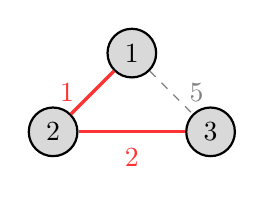
\begin{tikzpicture}[every node/.style={circle, draw, minimum size=0.5cm, thick}]
        \node[fill=gray!30] (1) at (0, 1) {1};
        \node[fill=gray!30] (2) at (-1, 0) {2};
        \node[fill=gray!30] (3) at (1, 0) {3};
        \draw[very thick, red!80] (1) -- node[left, draw=none, fill=none] {1} (2);
        \draw[dashed, gray] (1) -- node[right, draw=none, fill=none] {5} (3);
        \draw[very thick, red!80] (2) -- node[below, draw=none, fill=none] {2} (3);
    \end{tikzpicture}

    \vspace{0.2cm}
    \footnotesize
    \raggedright
    Remove menor aresta (peso 2). Visita o nó 3. Todos conectados! Custo total: 3.
\end{minipage}

\vspace{0.3cm}

\paragraph{Implementação: }\mbox{}\\
\textbf{Python: }
\begin{lstlisting}[language=Python]
import heapq

def prim(n, adj):
    # adj[u] = lista de tuplas (peso, v)
    visitado = [False] * n
    pq = [(0, 0)] # (peso, vertice)
    custo_total = 0
    
    while pq:
        peso, u = heapq.heappop(pq)
        
        if visitado[u]:
            continue
            
        visitado[u] = True
        custo_total += peso
        
        for peso_vizinho, v in adj[u]:
            if not visitado[v]:
                heapq.heappush(pq, (peso_vizinho, v))
                
    return custo_total
\end{lstlisting}

\vspace{0.3cm}
\textbf{C++:}
\begin{lstlisting}[language=C++]
int prim(int n, const vector<vector<pair<int, int>>>& adj) {
    vector<bool> visitado(n, false);
    priority_queue<pair<int, int>, vector<pair<int, int>>, greater<pair<int, int>>> pq;
    
    pq.push({0, 0}); // {peso, vertice}
    int custoTotal = 0;
    
    while (!pq.empty()) {
        int peso = pq.top().first;
        int u = pq.top().second;
        pq.pop();
        
        if (visitado[u]) continue;
        visitado[u] = true;
        custoTotal += peso;
        
        for (auto& edge : adj[u]) {
            int pesoVizinho = edge.first;
            int v = edge.second;
            
            if (!visitado[v]) {
                pq.push({pesoVizinho, v});
            }
        }
    }
    return custoTotal;
}
\end{lstlisting}
\newpage

\subsection{Algoritmos de Componentes Fortemente Conexas (SCCS) e Pontes de Articulação}
Um Componente Fortemente Conexo (SCC - \textit{Strongly Connected Component})
de um grafo direcionado é um subgrafo onde cada par de vértices é alcançável a
partir do outro. \subsubsection{Kosaraju (SCC com Duas DFS)}
O algoritmo de Kosaraju encontra todos os SCCs de um grafo direcionado
realizando duas DFS: a primeira no grafo original para ordenar os vértices por
tempo de término (usando uma pilha), e a segunda no grafo transposto (com as
arestas invertidas) na ordem da pilha. Sua complexidade de tempo é
$\mathcal{O}(V + E)$.

\paragraph{Pseudo-Código: }\mbox{}\\
\begin{algorithm}[H]
    \SetAlgoLined
    \SetKwFunction{Kosaraju}{Kosaraju}
    \SetKwProg{Fn}{Função}{:}{}

    \Fn{\Kosaraju{$adj, V$}}{
        $visitado \gets$ vetor falso de tamanho $V$\;
        $pilha \gets \emptyset$\;

        \For{$i \gets 0$ \Ate $V - 1$}{
            \Se{$\neg visitado[i]$}{
                \text{DFS1($i$, adj, visitado, pilha)}\;
            }
        }

        $adjT \gets$ \text{inverter todas as arestas de } $adj$\;
        $visitado \gets$ limpar visitados\;
        $sccs \gets \emptyset$\;

        \While{$pilha$ não vazia}{
            $u \gets pilha.pop()$\;
            \Se{$\neg visitado[u]$}{
                $componente \gets \emptyset$\;
                \text{DFS2($u$, adjT, visitado, componente)}\;
                $sccs.add(componente)$\;
            }
        }
        \Retorna $sccs$\;
    }
    \caption{Algoritmo de Kosaraju}
\end{algorithm}

Veja o Kosaraju funcionando em duas etapas:\\ \vspace{0.5cm} \noindent
\begin{minipage}[t]{0.31\textwidth}
    \centering
    \textbf{Passo 1: 1ª DFS (Original)}\\
    \vspace{0.2cm}
    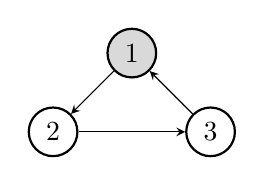
\begin{tikzpicture}[every node/.style={circle, draw, minimum size=0.5cm, thick}, >=stealth]
        \node[fill=gray!30] (1) at (0, 1) {1};
        \node (2) at (-1, 0) {2};
        \node (3) at (1, 0) {3};
        \draw[->] (1) -- (2);
        \draw[->] (2) -- (3);
        \draw[->] (3) -- (1);
    \end{tikzpicture}

    \vspace{0.2cm}
    \footnotesize
    \raggedright
    Executa DFS no grafo original e armazena os nós na pilha por tempo de término.
\end{minipage}%
\hfill
%
\begin{minipage}[t]{0.31\textwidth}
    \centering
    \textbf{Passo 2: Grafo Transposto}\\
    \vspace{0.2cm}
    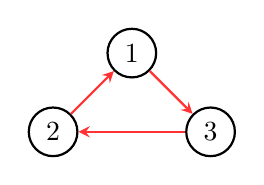
\begin{tikzpicture}[every node/.style={circle, draw, minimum size=0.5cm, thick}, >=stealth]
        \node (1) at (0, 1) {1};
        \node (2) at (-1, 0) {2};
        \node (3) at (1, 0) {3};
        \draw[->, red!80, thick] (2) -- (1);
        \draw[->, red!80, thick] (3) -- (2);
        \draw[->, red!80, thick] (1) -- (3);
    \end{tikzpicture}

    \vspace{0.2cm}
    \footnotesize
    \raggedright
    Inverte todas as arestas do grafo original para formar o grafo transposto ($adjT$).
\end{minipage}%
\hfill
%
\begin{minipage}[t]{0.31\textwidth}
    \centering
    \textbf{Passo 3: 2ª DFS (SCCs)}\\
    \vspace{0.2cm}
    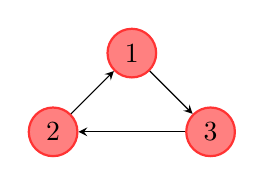
\begin{tikzpicture}[every node/.style={circle, draw, minimum size=0.5cm, thick}, >=stealth]
        \node[fill=red!50, draw=red!80] (1) at (0, 1) {1};
        \node[fill=red!50, draw=red!80] (2) at (-1, 0) {2};
        \node[fill=red!50, draw=red!80] (3) at (1, 0) {3};
        \draw[->] (2) -- (1);
        \draw[->] (3) -- (2);
        \draw[->] (1) -- (3);
    \end{tikzpicture}

    \vspace{0.2cm}
    \footnotesize
    \raggedright
    Executa DFS baseada na pilha. Cada árvore alcançada forma um SCC isolado.
\end{minipage}

\vspace{0.3cm}

\paragraph{Implementação: }\mbox{}\\
\textbf{Python: }
\begin{lstlisting}[language=Python]
def kosaraju(n, adj):
    def dfs1(u):
        visitado[u] = True
        for v in adj[u]:
            if not visitado[v]:
                dfs1(v)
        pilha.append(u)

    def dfs2(u, comp):
        visitado[u] = True
        comp.append(u)
        for v in adjT[u]:
            if not visitado[v]:
                dfs2(v, comp)

    visitado = [False] * n
    pilha = []
    for i in range(n):
        if not visitado[i]:
            dfs1(i)
            
    adjT = [[] for _ in range(n)]
    for u in range(n):
        for v in adj[u]:
            adjT[v].append(u)
            
    visitado = [False] * n
    sccs = []
    while pilha:
        u = pilha.pop()
        if not visitado[u]:
            comp = []
            dfs2(u, comp)
            sccs.append(comp)
    return sccs
\end{lstlisting}

\vspace{0.3cm}
\textbf{C++:}
\begin{lstlisting}[language=C++]
void dfs1(int u, const vector<vector<int>>& adj, vector<bool>& vis, stack<int>& st) {
    vis[u] = true;
    for (int v : adj[u]) if (!vis[v]) dfs1(v, adj, vis, st);
    st.push(u);
}

void dfs2(int u, const vector<vector<int>>& adjT, vector<bool>& vis, vector<int>& comp) {
    vis[u] = true;
    comp.push_back(u);
    for (int v : adjT[u]) if (!vis[v]) dfs2(v, adjT, vis, comp);
}

vector<vector<int>> kosaraju(int n, const vector<vector<int>>& adj) {
    vector<bool> vis(n, false);
    stack<int> st;
    for (int i = 0; i < n; ++i) if (!vis[i]) dfs1(i, adj, vis, st);
    
    vector<vector<int>> adjT(n);
    for (int u = 0; u < n; ++u)
        for (int v : adj[u]) adjT[v].push_back(u);
        
    fill(vis.begin(), vis.end(), false);
    vector<vector<int>> sccs;
    while (!st.empty()) {
        int u = st.top(); st.pop();
        if (!vis[u]) {
            vector<int> comp;
            dfs2(u, adjT, vis, comp);
            sccs.push_back(comp);
        }
    }
    return sccs;
}
\end{lstlisting}
\newpage \subsubsection{Tarjan (SCC em Uma Única Passada)}
O algoritmo de Tarjan encontra os SCCs utilizando apenas uma única DFS. Ele
mantém o tempo de descoberta de cada vértice (\textit{tin}) e o menor tempo
alcançável (\textit{low}). Utiliza uma pilha auxiliar para agrupar os nós
pertencentes ao mesmo componente conexo. Complexidade de tempo: $\mathcal{O}(V
    + E)$.

\paragraph{Pseudo-Código: }\mbox{}\\
\begin{algorithm}[H]
    \SetAlgoLined
    \SetKwFunction{Tarjan}{TarjanDFS}
    \SetKwProg{Fn}{Função}{:}{}

    \Fn{\Tarjan{$u, tin, low, pilha, naPilha, adj$}}{
        $tin[u] \gets low[u] \gets timer$\;
        $timer \gets timer + 1$\;
        $pilha.push(u)$\;
        $naPilha[u] \gets \text{true}$\;

        \For{$v \in adj[u]$}{
            \Se{$tin[v] == 0$}{
                \Tarjan{$v, tin, low, pilha, naPilha, adj$}\;
                $low[u] \gets \min(low[u], low[v])$\;
            }
            \Se{$naPilha[v]$}{
                $low[u] \gets \min(low[u], tin[v])$\;
            }
        }

        \Se{$low[u] == tin[u]$}{
            \text{// Encontrou a raiz de um SCC}\;
            \While{$topo \neq u$}{
                $topo \gets pilha.pop()$\;
                $naPilha[topo] \gets \text{false}$\;
                \text{adiciona $topo$ ao SCC atual}\;
            }
        }
    }
    \caption{Algoritmo de Tarjan para SCC}
\end{algorithm}

Veja o Tarjan utilizando tempos de descoberta e valores de \textit{low}:\\
\vspace{0.5cm} \noindent
\begin{minipage}[t]{0.31\textwidth}
    \centering
    \textbf{Passo 1: Descoberta ($tin, low$)}\\
    \vspace{0.2cm}
    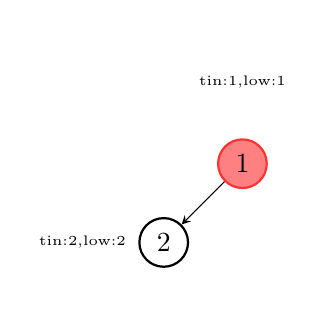
\begin{tikzpicture}[every node/.style={circle, draw, minimum size=0.5cm, thick}, >=stealth]
        \node[fill=red!50, draw=red!80, label=above:{\tiny tin:1,low:1}] (1) at (0, 1) {1};
        \node[label=left:{\tiny tin:2,low:2}] (2) at (-1, 0) {2};
        \draw[->] (1) -- (2);
    \end{tikzpicture}

    \vspace{0.2cm}
    \footnotesize
    \raggedright
    Visita o nó 1, define $tin[1]=low[1]=1$ e empilha. Vai para o nó 2.
\end{minipage}%
\hfill
%
\begin{minipage}[t]{0.31\textwidth}
    \centering
    \textbf{Passo 2: Back-edge e Low}\\
    \vspace{0.2cm}
    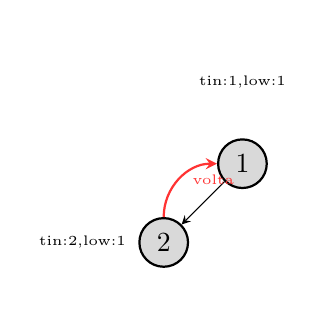
\begin{tikzpicture}[every node/.style={circle, draw, minimum size=0.5cm, thick}, >=stealth]
        \node[fill=gray!30, label=above:{\tiny tin:1,low:1}] (1) at (0, 1) {1};
        \node[fill=gray!30, label=left:{\tiny tin:2,low:1}] (2) at (-1, 0) {2};
        \draw[->] (1) -- (2);
        \draw[->, bend left=45, red!80, thick] (2) to node[right, draw=none, fill=none] {\tiny volta} (1);
    \end{tikzpicture}

    \vspace{0.2cm}
    \footnotesize
    \raggedright
    Aresta de retorno de 2 para 1 atualiza $low[2] = \min(low[2], tin[1]) = 1$.
\end{minipage}%
\hfill
%
\begin{minipage}[t]{0.31\textwidth}
    \centering
    \textbf{Passo 3: Raiz do SCC}\\
    \vspace{0.2cm}
    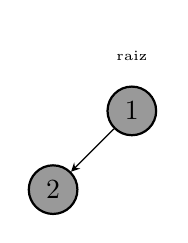
\begin{tikzpicture}[every node/.style={circle, draw, minimum size=0.5cm, thick}, >=stealth]
        \node[fill=gray!80, label=above:{\tiny raiz}] (1) at (0, 1) {1};
        \node[fill=gray!80] (2) at (-1, 0) {2};
        \draw[->] (1) -- (2);
    \end{tikzpicture}

    \vspace{0.2cm}
    \footnotesize
    \raggedright
    Como $low[1] == tin[1]$, 1 é raiz de um SCC. Desempilha os nós até 1.
\end{minipage}

\vspace{0.3cm}

\paragraph{Implementação: }\mbox{}\\
\textbf{C++:}
\begin{lstlisting}[language=C++]
int timer = 0;
void tarjanDFS(int u, const vector<vector<int>>& adj, vector<int>& tin, vector<int>& low, stack<int>& st, vector<bool>& inStack, vector<vector<int>>& sccs) {
    tin[u] = low[u] = ++timer;
    st.push(u);
    inStack[u] = true;
    
    for (int v : adj[u]) {
        if (tin[v] == -1) {
            tarjanDFS(v, adj, tin, low, st, inStack, sccs);
            low[u] = min(low[u], low[v]);
        } else if (inStack[v]) {
            low[u] = min(low[u], tin[v]);
        }
    }
    
    if (low[u] == tin[u]) {
        vector<int> comp;
        while (true) {
            int v = st.top(); st.pop();
            inStack[v] = false;
            comp.push_back(v);
            if (u == v) break;
        }
        sccs.push_back(comp);
    }
}
\end{lstlisting}
\newpage

\subsection{Algoritmos de Fluxo Máximo e Emparelhamento Bipartido}
Problemas de fluxo máximo modelam redes de transporte onde cada aresta possui
uma capacidade máxima. O objetivo é enviar o máximo de "fluxo" possível de uma
fonte ($S$) até um sumidouro ($T$). \subsubsection{Dinic (Fluxo Máximo Eficiente)}
O algoritmo de Dinic utiliza o conceito de \textit{grafo de níveis} (construído
via BFS) para encontrar caminhos de aumento e \textit{fluxos bloqueantes}
(encontrados via DFS) em camadas. Sua complexidade de tempo é $\mathcal{O}(V^2
    E)$, sendo extremamente rápido em grafos gerais.

\paragraph{Pseudo-Código: }\mbox{}\\
\begin{algorithm}[H]
    \SetAlgoLined
    \SetKwFunction{Dinic}{Dinic}
    \SetKwProg{Fn}{Função}{:}{}

    \Fn{\Dinic{$s, t, adj$}}{
        $fluxoMaximo \gets 0$\;
        \While{\text{BFS constrói o grafo de níveis a partir de } $s$ \text{ até } $t$}{
            \While{\text{encontrar caminho de fluxo bloqueante com DFS}}{
                $fluxoMaximo \gets fluxoMaximo + \text{fluxoEncontrado}$\;
            }
        }
        \Retorna $fluxoMaximo$\;
    }
    \caption{Algoritmo de Dinic}
\end{algorithm}

Veja o Dinic construindo o grafo de níveis e encontrando o fluxo bloqueante:\\
\vspace{0.5cm} \noindent
\begin{minipage}[t]{0.31\textwidth}
    \centering
    \textbf{Passo 1: Rede Residual}\\
    \vspace{0.2cm}
    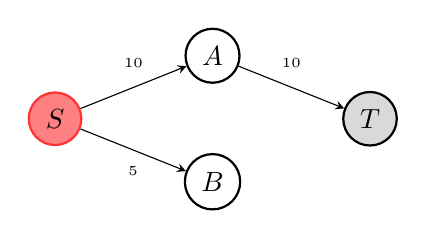
\begin{tikzpicture}[every node/.style={circle, draw, minimum size=0.5cm, thick}, >=stealth]
        \node[fill=red!50, draw=red!80] (S) at (-1, 0) {$S$};
        \node (A) at (1, 0.8) {$A$};
        \node (B) at (1, -0.8) {$B$};
        \node[fill=gray!30] (T) at (3, 0) {$T$};
        \draw[->] (S) -- node[above, draw=none, fill=none] {\tiny 10} (A);
        \draw[->] (S) -- node[below, draw=none, fill=none] {\tiny 5} (B);
        \draw[->] (A) -- node[above, draw=none, fill=none] {\tiny 10} (T);
    \end{tikzpicture}

    \vspace{0.2cm}
    \footnotesize
    \raggedright
    Rede inicial com capacidades nas arestas entre a fonte $S$ e o sumidouro $T$.
\end{minipage}%
\hfill
%
\begin{minipage}[t]{0.31\textwidth}
    \centering
    \textbf{Passo 2: Grafo de Níveis (BFS)}\\
    \vspace{0.2cm}
    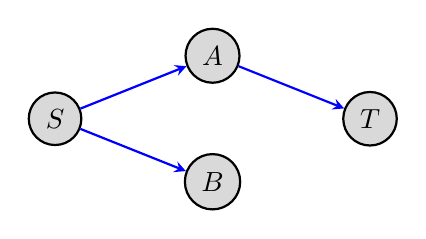
\begin{tikzpicture}[every node/.style={circle, draw, minimum size=0.5cm, thick}, >=stealth]
        \node[fill=gray!30] (S) at (-1, 0) {$S$};
        \node[fill=gray!30] (A) at (1, 0.8) {$A$};
        \node[fill=gray!30] (B) at (1, -0.8) {$B$};
        \node[fill=gray!30] (T) at (3, 0) {$T$};
        \draw[->, blue, thick] (S) -- (A);
        \draw[->, blue, thick] (S) -- (B);
        \draw[->, blue, thick] (A) -- (T);
    \end{tikzpicture}

    \vspace{0.2cm}
    \footnotesize
    \raggedright
    BFS atribui níveis aos nós ($level[S]=0, level[A]=1, level[T]=2$).
\end{minipage}%
\hfill
%
\begin{minipage}[t]{0.31\textwidth}
    \centering
    \textbf{Passo 3: Fluxo Bloqueante (DFS)}\\
    \vspace{0.2cm}
    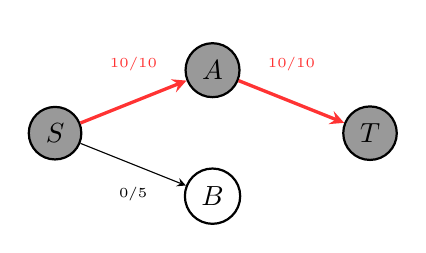
\begin{tikzpicture}[every node/.style={circle, draw, minimum size=0.5cm, thick}, >=stealth]
        \node[fill=gray!80] (S) at (-1, 0) {$S$};
        \node[fill=gray!80] (A) at (1, 0.8) {$A$};
        \node (B) at (1, -0.8) {$B$};
        \node[fill=gray!80] (T) at (3, 0) {$T$};
        \draw[->, red!80, very thick] (S) -- node[above, draw=none, fill=none] {\tiny 10/10} (A);
        \draw[->] (S) -- node[below, draw=none, fill=none] {\tiny 0/5} (B);
        \draw[->, red!80, very thick] (A) -- node[above, draw=none, fill=none] {\tiny 10/10} (T);
    \end{tikzpicture}

    \vspace{0.2cm}
    \footnotesize
    \raggedright
    DFS envia fluxo pelas camadas até que nenhuma rota adicional seja possível.
\end{minipage}

\vspace{0.3cm}

\paragraph{Implementação: }\mbox{}\\
\textbf{C++ (Estrutura Completa de Dinic):}
\begin{lstlisting}[language=C++]
struct Edge {
    int to;
    long long cap;
    long long flow;
    int rev;
};

struct Dinic {
    int n;
    vector<vector<Edge>> adj;
    vector<int> level, ptr;

    Dinic(int n) : n(n), adj(n), level(n), ptr(n) {}

    void add_edge(int from, int to, long long cap) {
        adj[from].push_back({to, cap, 0, (int)adj[to].size()});
        adj[to].push_back({from, 0, 0, (int)adj[from].size() - 1});
    }

    bool bfs(int s, int t) {
        fill(level.begin(), level.end(), -1);
        level[s] = 0;
        queue<int> q;
        q.push(s);
        while (!q.empty()) {
            int v = q.front();
            q.pop();
            for (auto& edge : adj[v]) {
                if (edge.cap - edge.flow > 0 && level[edge.to] == -1) {
                    level[edge.to] = level[v] + 1;
                    q.push(edge.to);
                }
            }
        }
        return level[t] != -1;
    }

    long long dfs(int v, int t, long long pushed) {
        if (pushed == 0) return 0;
        if (v == t) return pushed;
        for (int& cid = ptr[v]; cid < adj[v].size(); ++cid) {
            auto& edge = adj[v][cid];
            int tr = edge.to;
            if (level[v] + 1 != level[tr] || edge.cap - edge.flow == 0) continue;
            long long tr_pushed = dfs(tr, t, min(pushed, edge.cap - edge.flow));
            if (tr_pushed == 0) continue;
            edge.flow += tr_pushed;
            adj[tr][edge.rev].flow -= tr_pushed;
            return tr_pushed;
        }
        return 0;
    }

    long long max_flow(int s, int t) {
        long long flow = 0;
        while (bfs(s, t)) {
            fill(ptr.begin(), ptr.end(), 0);
            while (long long pushed = dfs(s, t, 1e18)) {
                flow += pushed;
            }
        }
        return flow;
    }
};
\end{lstlisting}
\newpage
\subsubsection{Algoritmo de Kuhn (Emparelhamento Bipartido Máximo)}
O emparelhamento bipartido máximo (\textit{Maximum Bipartite Matching})
encontra o maior conjunto possível de arestas em um grafo bipartido onde
nenhuma aresta compartilha um vértice final. O Algoritmo de Kuhn resolve isso
utilizando caminhos de aumento via DFS de forma muito elegante. Complexidade:
$\mathcal{O}(V \cdot E)$.

\paragraph{Pseudo-Código: }\mbox{}\\
\begin{algorithm}[H]
    \SetAlgoLined
    \SetKwFunction{Kuhn}{try\_kuhn}
    \SetKwProg{Fn}{Função}{:}{}

    \Fn{\Kuhn{$v, adj, visitado, emparelhamento$}}{
        \If{$visitado[v]$}{
            \Retorna \text{falso}\;
        }
        $visitado[v] \gets \text{true}$\;
        \ParaCada{$to \in adj[v]$}{
            \Se{$emparelhamento[to] == -1$ \textbf{ou} \Kuhn{$emparelhamento[to], adj, visitado, emparelhamento$}}{
                $emparelhamento[to] \gets v$\;
                \Retorna \text{verdadeiro}\;
            }
        }
        \Retorna \text{falso}\;
    }
    \caption{Algoritmo de Kuhn para Emparelhamento Bipartido}
\end{algorithm}

Veja o Algoritmo de Kuhn encontrando o emparelhamento máximo:\\ \vspace{0.5cm}
\noindent
\begin{minipage}[t]{0.31\textwidth}
    \centering
    \textbf{Passo 1: Lados $L$ e $R$}\\
    \vspace{0.2cm}
    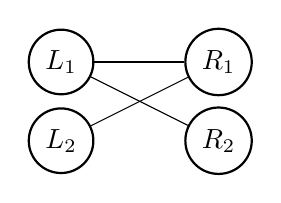
\begin{tikzpicture}[every node/.style={circle, draw, minimum size=0.5cm, thick}, >=stealth]
        \node (L1) at (0, 0.5) {$L_1$};
        \node (L2) at (0, -0.5) {$L_2$};
        \node (R1) at (2, 0.5) {$R_1$};
        \node (R2) at (2, -0.5) {$R_2$};
        \draw (L1) -- (R1);
        \draw (L1) -- (R2);
        \draw (L2) -- (R1);
    \end{tikzpicture}

    \vspace{0.2cm}
    \footnotesize
    \raggedright
    Grafo dividido em dois conjuntos disjuntos $L$ e $R$. Nenhum casamento inicial.
\end{minipage}%
\hfill
%
\begin{minipage}[t]{0.31\textwidth}
    \centering
    \textbf{Passo 2: Tentativa de Casamento}\\
    \vspace{0.2cm}
    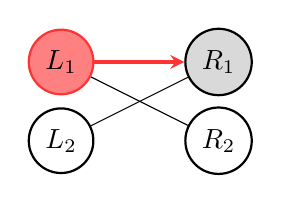
\begin{tikzpicture}[every node/.style={circle, draw, minimum size=0.5cm, thick}, >=stealth]
        \node[fill=red!50, draw=red!80] (L1) at (0, 0.5) {$L_1$};
        \node (L2) at (0, -0.5) {$L_2$};
        \node[fill=gray!30] (R1) at (2, 0.5) {$R_1$};
        \node (R2) at (2, -0.5) {$R_2$};
        \draw[->, very thick, red!80] (L1) -- (R1);
        \draw (L1) -- (R2);
        \draw (L2) -- (R1);
    \end{tikzpicture}

    \vspace{0.2cm}
    \footnotesize
    \raggedright
    $L_1$ tenta casar com $R_1$. Como $R_1$ está livre, o casamento é feito com sucesso.
\end{minipage}%
\hfill
%
\begin{minipage}[t]{0.31\textwidth}
    \centering
    \textbf{Passo 3: Caminho de Aumento}\\
    \vspace{0.2cm}
    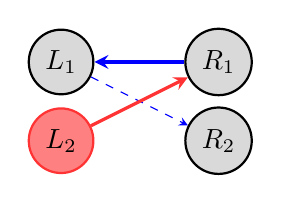
\begin{tikzpicture}[every node/.style={circle, draw, minimum size=0.5cm, thick}, >=stealth]
        \node[fill=gray!30] (L1) at (0, 0.5) {$L_1$};
        \node[fill=red!50, draw=red!80] (L2) at (0, -0.5) {$L_2$};
        \node[fill=gray!30] (R1) at (2, 0.5) {$R_1$};
        \node[fill=gray!30] (R2) at (2, -0.5) {$R_2$};
        \draw[->, dashed, blue] (L1) -- (R2);
        \draw[->, very thick, red!80] (L2) -- (R1);
        \draw[->, very thick, blue] (R1) -- (L1);
    \end{tikzpicture}

    \vspace{0.2cm}
    \footnotesize
    \raggedright
    $L_2$ quer $R_1$ (ocupado). $L_1$ muda para $R_2$, liberando $R_1$ para $L_2$!
\end{minipage}

\vspace{0.3cm}
\newpage
\paragraph{Implementação: }\mbox{}\\
\textbf{C++:}
\begin{lstlisting}[language=C++]
vector<vector<int>> adj;
vector<int> mt;
vector<bool> visited;

bool try_kuhn(int v) {
    if (visited[v]) return false;
    visited[v] = true;
    for (int to : adj[v]) {
        if (mt[to] == -1 || try_kuhn(mt[to])) {
            mt[to] = v;
            return true;
        }
    }
    return false;
}

int max_bipartite_matching(int n, int m) {
    //n = nos do lado esquerdo, m = nos do lado direito
    mt.assign(m, -1);
    int count = 0;
    for (int v = 0; v < n; ++v) {
        visited.assign(n, false);
        if (try_kuhn(v)) ++count;
    }
    return count;
}
\end{lstlisting}
\newpage

\subsection{Algoritmos mais Complexos}
\subsubsection{LCA - Lowest Common Ancestor (Menor Ancestral Comum)}
O LCA de dois nós $u$ e $v$ em uma árvore enraizada é o nó mais profundo que é
ancestral de ambos. O método de \textit{Binary Lifting} (Içamento Binário)
pré-calcula os ancestrais de potências de 2 em $\mathcal{O}(N \log N)$,
permitindo responder a cada consulta de LCA em $\mathcal{O}(\log N)$.

Veja o LCA por Içamento Binário em ação:\\ \vspace{0.5cm} \noindent
\begin{minipage}[t]{0.31\textwidth}
    \centering
    \textbf{Passo 1: Árvore Enraizada}\\
    \vspace{0.2cm}
    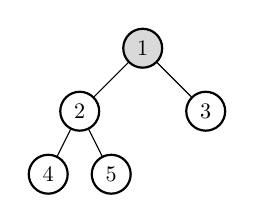
\begin{tikzpicture}[every node/.style={circle, draw, minimum size=0.5cm, thick}, scale=0.8, every node/.append style={transform shape}, >=stealth]
        \node[fill=gray!30] (1) at (1, 2) {1};
        \node (2) at (0, 1) {2};
        \node (3) at (2, 1) {3};
        \node (4) at (-0.5, 0) {4};
        \node (5) at (0.5, 0) {5};
        \draw (1) -- (2);
        \draw (1) -- (3);
        \draw (2) -- (4);
        \draw (2) -- (5);
    \end{tikzpicture}

    \vspace{0.2cm}
    \footnotesize
    \raggedright
    Árvore com 5 nós. O nó 1 é definido como a raiz.
\end{minipage}%
\hfill
%
\begin{minipage}[t]{0.31\textwidth}
    \centering
    \textbf{Passo 2: Pré-cálculo ($up$)}\\
    \vspace{0.2cm}
    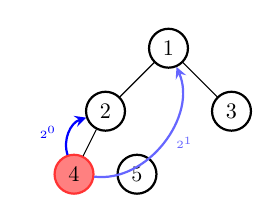
\begin{tikzpicture}[every node/.style={circle, draw, minimum size=0.5cm, thick}, scale=0.8, every node/.append style={transform shape}, >=stealth]
        \node (1) at (1, 2) {1};
        \node (2) at (0, 1) {2};
        \node (3) at (2, 1) {3};
        \node[fill=red!50, draw=red!80] (4) at (-0.5, 0) {4};
        \node (5) at (0.5, 0) {5};
        \draw (1) -- (2);
        \draw (1) -- (3);
        \draw (2) -- (4);
        \draw[->, blue, thick, bend left=45] (4) to node[left, draw=none, fill=none] {\tiny $2^0$} (2);
        \draw[->, blue!60, thick, bend right=60] (4) to node[right, draw=none, fill=none] {\tiny $2^1$} (1);
    \end{tikzpicture}

    \vspace{0.2cm}
    \footnotesize
    \raggedright
    Armazena ancestrais de potências de 2 ($up[4][0]=2, up[4][1]=1$).
\end{minipage}%
\hfill
%
\begin{minipage}[t]{0.31\textwidth}
    \centering
    \textbf{Passo 3: Consulta de LCA}\\
    \vspace{0.2cm}
    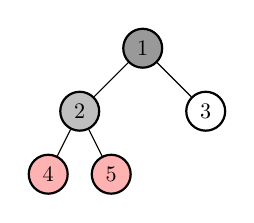
\begin{tikzpicture}[every node/.style={circle, draw, minimum size=0.5cm, thick}, scale=0.8, every node/.append style={transform shape}, >=stealth]
        \node[fill=gray!80] (1) at (1, 2) {1};
        \node[fill=gray!50] (2) at (0, 1) {2};
        \node (3) at (2, 1) {3};
        \node[fill=red!30] (4) at (-0.5, 0) {4};
        \node[fill=red!30] (5) at (0.5, 0) {5};
        \draw (1) -- (2);
        \draw (1) -- (3);
        \draw (2) -- (4);
        \draw (2) -- (5);
    \end{tikzpicture}

    \vspace{0.2cm}
    \footnotesize
    \raggedright
    O LCA entre os nós 4 e 5 é o nó 2 (ancestral comum mais profundo).
\end{minipage}

\vspace{0.3cm}

\paragraph{Implementação: }\mbox{}\\
\textbf{C++:}
\begin{lstlisting}[language=C++]
int n, l;
vector<vector<int>> adj;
vector<vector<int>> up;
vector<int> tin, tout;
int timer;

void dfs(int v, int p) {
    tin[v] = ++timer;
    up[v][0] = p;
    for (int i = 1; i <= l; ++i)
        up[v][i] = up[up[v][i - 1]][i - 1];
    for (int u : adj[v]) {
        if (u != p) dfs(u, v);
    }
    tout[v] = ++timer;
}

bool is_ancestor(int u, int v) {
    return tin[u] <= tin[v] && tout[u] >= tout[v];
}

int lca(int u, int v) {
    if (is_ancestor(u, v)) return u;
    if (is_ancestor(v, u)) return v;
    for (int i = l; i >= 0; --i) {
        if (!is_ancestor(up[u][i], v))
            u = up[u][i];
    }
    return up[u][0];
}

void preprocess(int root) {
    tin.resize(n); tout.resize(n);
    timer = 0;
    l = ceil(log2(n));
    up.assign(n, vector<int>(l + 1));
    dfs(root, root);
}
\end{lstlisting}
\newpage
\subsubsection{Segment Tree (Árvore de Segmentos)}
A Segment Tree é uma estrutura de dados binária que armazena intervalos ou
segmentos. Ela permite realizar consultas de intervalo (como soma, mínimo,
máximo) e atualizações de elementos ou intervalos em tempo $\mathcal{O}(\log
    N)$.

Veja a Segment Tree construída sobre um vetor de 4 elementos:\\ \vspace{0.5cm}
\noindent
\begin{minipage}[t]{0.31\textwidth}
    \centering
    \textbf{Passo 1: Vetor Base}\\
    \vspace{0.2cm}
    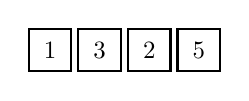
\begin{tikzpicture}[every node/.style={rectangle, draw, minimum size=0.6cm, thick}, scale=0.9, every node/.append style={transform shape}]
        \node (a1) at (0,0) {1};
        \node (a2) at (0.7,0) {3};
        \node (a3) at (1.4,0) {2};
        \node (a4) at (2.1,0) {5};
    \end{tikzpicture}

    \vspace{0.4cm}
    \footnotesize
    \raggedright
    Vetor inicial com 4 elementos ($N=4$).
\end{minipage}%
\hfill
%
\begin{minipage}[t]{0.31\textwidth}
    \centering
    \textbf{Passo 2: Árvore Binária}\\
    \vspace{0.2cm}
    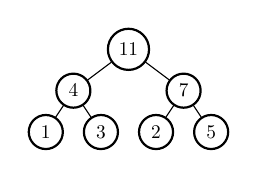
\begin{tikzpicture}[every node/.style={circle, draw, minimum size=0.5cm, thick}, scale=0.7, every node/.append style={transform shape}, >=stealth]
        \node (root) at (1, 1.5) {11};
        \node (l1) at (0, 0.75) {4};
        \node (r1) at (2, 0.75) {7};
        \node (ll) at (-0.5, 0) {1};
        \node (lr) at (0.5, 0) {3};
        \node (rl) at (1.5, 0) {2};
        \node (rr) at (2.5, 0) {5};
        \draw (root) -- (l1);
        \draw (root) -- (r1);
        \draw (l1) -- (ll);
        \draw (l1) -- (lr);
        \draw (r1) -- (rl);
        \draw (r1) -- (rr);
    \end{tikzpicture}

    \vspace{0.2cm}
    \footnotesize
    \raggedright
    Cada nó pai armazena a soma dos filhos (Total = 11, total de 7 nós).
\end{minipage}%
\hfill
%
\begin{minipage}[t]{0.31\textwidth}
    \centering
    \textbf{Passo 3: Atualização}\\
    \vspace{0.2cm}
    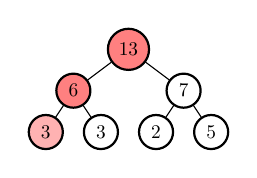
\begin{tikzpicture}[every node/.style={circle, draw, minimum size=0.5cm, thick}, scale=0.7, every node/.append style={transform shape}, >=stealth]
        \node[fill=red!50] (root) at (1, 1.5) {13};
        \node[fill=red!50] (l1) at (0, 0.75) {6};
        \node (r1) at (2, 0.75) {7};
        \node[fill=red!30] (ll) at (-0.5, 0) {3};
        \node (lr) at (0.5, 0) {3};
        \node (rl) at (1.5, 0) {2};
        \node (rr) at (2.5, 0) {5};
        \draw (root) -- (l1);
        \draw (root) -- (r1);
        \draw (l1) -- (ll);
        \draw (l1) -- (lr);
        \draw (r1) -- (rl);
        \draw (r1) -- (rr);
    \end{tikzpicture}

    \vspace{0.2cm}
    \footnotesize
    \raggedright
    Atualiza a posição 0 de 1 para 3. Propaga os valores em $\mathcal{O}(\log N)$.
\end{minipage}

\vspace{0.3cm}

\paragraph{Implementação: }\mbox{}\\
\textbf{C++:}
\begin{lstlisting}[language=C++]
struct SegTree {
    int n;
    vector<long long> tree;

    SegTree(int n) : n(n), tree(4 * n, 0) {}

    void update(int node, int start, int end, int idx, long long val) {
        if (start == end) {
            tree[node] = val;
            return;
        }
        int mid = (start + end) / 2;
        if (idx <= mid) update(2 * node, start, mid, idx, val);
        else update(2 * node + 1, mid + 1, end, idx, val);
        tree[node] = tree[2 * node] + tree[2 * node + 1];
    }

    long long query(int node, int start, int end, int l, int r) {
        if (r < start || end < l) return 0;
        if (l <= start && end <= r) return tree[node];
        int mid = (start + end) / 2;
        return query(2 * node, start, mid, l, r) + query(2 * node + 1, mid + 1, end, l, r);
    }
};
\end{lstlisting}
\newpage
\subsubsection{HLD - Heavy-Light Decomposition}
O HLD decompõe uma árvore em uma coleção de caminhos disjuntos (cadeias). Ele
classifica as arestas em \textit{Heavy} (para o filho com a maior subárvore) e
\textit{Light}. Isso garante que qualquer caminho entre dois nós na árvore
cruza no máximo $\mathcal{O}(\log N)$ arestas \textit{light}. Combinado com uma
Segment Tree, permite resolver consultas complexas em caminhos de árvores em
$\mathcal{O}(\log^2 N)$.

Veja a Decomposição Heavy-Light em uma árvore de 6 nós:\\ \vspace{0.5cm}
\noindent
\begin{minipage}[t]{0.31\textwidth}
    \centering
    \textbf{Passo 1: Tamanho Subárvores}\\
    \vspace{0.2cm}
    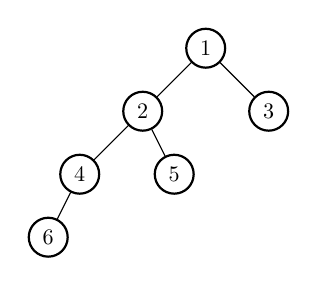
\begin{tikzpicture}[every node/.style={circle, draw, minimum size=0.5cm, thick}, scale=0.8, every node/.append style={transform shape}, >=stealth]
        \node (1) at (1, 2) {1};
        \node (2) at (0, 1) {2};
        \node (3) at (2, 1) {3};
        \node (4) at (-1, 0) {4};
        \node (5) at (0.5, 0) {5};
        \node (6) at (-1.5, -1) {6};
        \draw (1) -- (2);
        \draw (1) -- (3);
        \draw (2) -- (4);
        \draw (2) -- (5);
        \draw (4) -- (6);
    \end{tikzpicture}

    \vspace{0.2cm}
    \footnotesize
    \raggedright
    Calcula o tamanho das subárvores de cada filho para determinar a aresta pesada.
\end{minipage}%
\hfill
%
\begin{minipage}[t]{0.31\textwidth}
    \centering
    \textbf{Passo 2: Arestas Heavy}\\
    \vspace{0.2cm}
    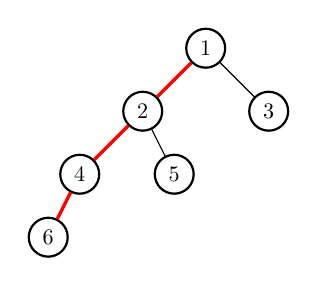
\begin{tikzpicture}[every node/.style={circle, draw, minimum size=0.5cm, thick}, scale=0.8, every node/.append style={transform shape}, >=stealth]
        \node (1) at (1, 2) {1};
        \node (2) at (0, 1) {2};
        \node (3) at (2, 1) {3};
        \node (4) at (-1, 0) {4};
        \node (5) at (0.5, 0) {5};
        \node (6) at (-1.5, -1) {6};
        \draw[red, very thick] (1) -- (2);
        \draw (1) -- (3);
        \draw[red, very thick] (2) -- (4);
        \draw (2) -- (5);
        \draw[red, very thick] (4) -- (6);
    \end{tikzpicture}

    \vspace{0.2cm}
    \footnotesize
    \raggedright
    Arestas pesadas (\textit{heavy}, em vermelho) vão para o filho com maior subárvore.
\end{minipage}%
\hfill
%
\begin{minipage}[t]{0.31\textwidth}
    \centering
    \textbf{Passo 3: Cadeias Disjuntas}\\
    \vspace{0.2cm}
    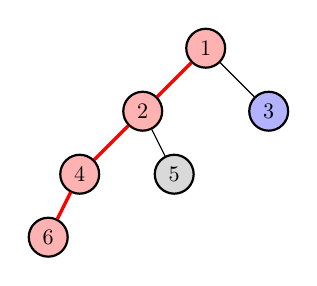
\begin{tikzpicture}[every node/.style={circle, draw, minimum size=0.5cm, thick}, scale=0.8, every node/.append style={transform shape}, >=stealth]
        \node[fill=red!30] (1) at (1, 2) {1};
        \node[fill=red!30] (2) at (0, 1) {2};
        \node[fill=blue!30] (3) at (2, 1) {3};
        \node[fill=red!30] (4) at (-1, 0) {4};
        \node[fill=gray!30] (5) at (0.5, 0) {5};
        \node[fill=red!30] (6) at (-1.5, -1) {6};
        \draw[red, very thick] (1) -- (2);
        \draw (1) -- (3);
        \draw[red, very thick] (2) -- (4);
        \draw (2) -- (5);
        \draw[red, very thick] (4) -- (6);
    \end{tikzpicture}

    \vspace{0.2cm}
    \footnotesize
    \raggedright
    Árvore decomposta em cadeias lineares para consultas em $\mathcal{O}(\log^2 N)$.
\end{minipage}

\vspace{0.3cm}

\paragraph{Implementação: }\mbox{}\\
\textbf{C++:}
\begin{lstlisting}[language=C++]
vector<int> parent, depth, heavy, head, pos;
int cur_pos;

int dfs_hld(int v, vector<vector<int>>& adj) {
    int size = 1, max_c_size = 0;
    heavy[v] = -1;
    for (int u : adj[v]) {
        if (u != parent[v]) {
            parent[u] = v;
            depth[u] = depth[v] + 1;
            int c_size = dfs_hld(u, adj);
            size += c_size;
            if (c_size > max_c_size) {
                max_c_size = c_size;
                heavy[v] = u;
            }
        }
    }
    return size;
}

void decompose(int v, int h, vector<vector<int>>& adj) {
    head[v] = h;
    pos[v] = cur_pos++;
    if (heavy[v] != -1) decompose(heavy[v], h, adj);
    for (int u : adj[v]) {
        if (u != parent[v] && u != heavy[v]) decompose(u, u, adj);
    }
}

void init_hld(int n, vector<vector<int>>& adj) {
    parent.resize(n); depth.resize(n); heavy.assign(n, -1);
    head.resize(n); pos.resize(n);
    cur_pos = 0;
    dfs_hld(0, adj);
    decompose(0, 0, adj);
}
\end{lstlisting}
\newpage
\subsubsection{Centroid Decomposition (Decomposição em Centróide)}
A Decomposição em Centróide divide recursivamente uma árvore encontrando o
centróide (o nó cuja remoção deixa todas as subárvores com tamanho $\le N/2$).
Isso reduz a altura da árvore de decomposição para $\mathcal{O}(\log N)$, sendo
a ferramenta definitiva para resolver problemas de caminhos e distâncias entre
quaisquer pares de nós na árvore.

Veja a Decomposição em Centróide reduzindo a árvore:\\ \vspace{0.5cm} \noindent
\begin{minipage}[t]{0.31\textwidth}
    \centering
    \textbf{Passo 1: Árvore Original}\\
    \vspace{0.2cm}
    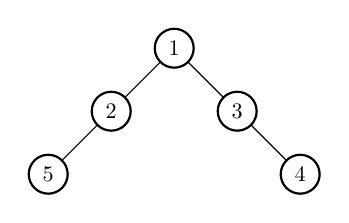
\begin{tikzpicture}[every node/.style={circle, draw, minimum size=0.5cm, thick}, scale=0.8, every node/.append style={transform shape}, >=stealth]
        \node (1) at (0, 1) {1};
        \node (2) at (-1, 0) {2};
        \node (3) at (1, 0) {3};
        \node (4) at (2, -1) {4};
        \node (5) at (-2, -1) {5};
        \draw (1) -- (2);
        \draw (1) -- (3);
        \draw (3) -- (4);
        \draw (2) -- (5);
    \end{tikzpicture}

    \vspace{0.2cm}
    \footnotesize
    \raggedright
    Árvore geral com 5 nós conectados.
\end{minipage}%
\hfill
%
\begin{minipage}[t]{0.31\textwidth}
    \centering
    \textbf{Passo 2: Achar Centróide}\\
    \vspace{0.2cm}
    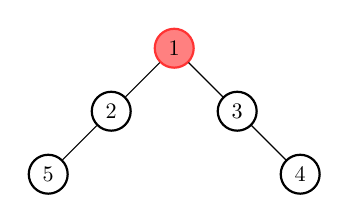
\begin{tikzpicture}[every node/.style={circle, draw, minimum size=0.5cm, thick}, scale=0.8, every node/.append style={transform shape}, >=stealth]
        \node[fill=red!50, draw=red!80] (1) at (0, 1) {1};
        \node (2) at (-1, 0) {2};
        \node (3) at (1, 0) {3};
        \node (4) at (2, -1) {4};
        \node (5) at (-2, -1) {5};
        \draw (1) -- (2);
        \draw (1) -- (3);
        \draw (3) -- (4);
        \draw (2) -- (5);
    \end{tikzpicture}

    \vspace{0.2cm}
    \footnotesize
    \raggedright
    Identifica o nó 1 como centróide (nenhuma subárvore excede $N/2$).
\end{minipage}%
\hfill
%
\begin{minipage}[t]{0.31\textwidth}
    \centering
    \textbf{Passo 3: Árvore de Centróides}\\
    \vspace{0.2cm}
    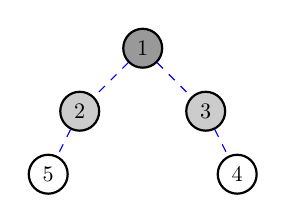
\begin{tikzpicture}[every node/.style={circle, draw, minimum size=0.5cm, thick}, scale=0.8, every node/.append style={transform shape}, >=stealth]
        \node[fill=gray!80] (1) at (0, 1) {1};
        \node[fill=gray!40] (2) at (-1, 0) {2};
        \node[fill=gray!40] (3) at (1, 0) {3};
        \node (4) at (1.5, -1) {4};
        \node (5) at (-1.5, -1) {5};
        \draw[dashed, blue] (1) -- (2);
        \draw[dashed, blue] (1) -- (3);
        \draw[dashed, blue] (3) -- (4);
        \draw[dashed, blue] (2) -- (5);
    \end{tikzpicture}

    \vspace{0.2cm}
    \footnotesize
    \raggedright
    Remove o centróide e repete recursivamente, formando a árvore de centróides (altura $\le \log N$).
\end{minipage}

\vspace{0.3cm}

\paragraph{Implementação: }\mbox{}\\
\textbf{C++:}
\begin{lstlisting}[language=C++]
vector<vector<int>> adj;
vector<bool> removed;
vector<int> sub_size;

void get_sub_size(int u, int p) {
    sub_size[u] = 1;
    for (int v : adj[u]) {
        if (v != p && !removed[v]) {
            get_sub_size(v, u);
            sub_size[u] += sub_size[v];
        }
    }
}

int get_centroid(int u, int p, int total) {
    for (int v : adj[u]) {
        if (v != p && !removed[v] && sub_size[v] > total / 2)
            return get_centroid(v, u, total);
    }
    return u;
}

void decompose(int u) {
    get_sub_size(u, u);
    int centroid = get_centroid(u, u, sub_size[u]);
    
    removed[centroid] = true;
    
    // Processa o centroide atual (ex: caminhos que passam por ele)
    
    for (int v : adj[centroid]) {
        if (!removed[v]) decompose(v);
    }
}
\end{lstlisting}